% Main chapter title
\chapter{Anwendung}

% Chapter Label
\label{application}

In diesem Kapitel beschäftigen wir uns mit der Anwendung der dünnbesetzten Hauptkomponentenanalyse auf Frequenzdaten einer Mühle. Dafür stehen uns Zeitreihen von Beschleunigungssensoren, welche die Vibration der Maschine messen, sowie akustische Daten, welche durch Mikrofone aufgezeichnet werden, zur Verfügung. Wir sind interessiert daran herauszufinden, ob sich mithilfe der Zeitreihen Aussagen über die Partikelgröße des Materials treffen lassen. Aufgrund der Beschaffenheit des Datensatzes sind viele überwachte Lernverfahren in diesem Zusammenhang unbrauchbar. Im Zuge einer explorativen Analyse kann daher eine Dimensionsreduktion sinnvoll sein. Dabei sind wir nicht unbedingt an der niedrigdimensionalen Repräsentation der Daten interessiert, sondern viel mehr an der Herausfilterung wichtiger Frequenzen. Idealerweise erhalten wir eine Trennung der Frequenzen je nachdem, ob sie durch die Maschine oder durch das Material erzeugt worden sind. Die Möglichkeit der Interpretation und die Konsistenz waren Anlass für die Verwendung der dünnbesetzten Hauptkomponentenanalyse in diesem Zusammenhang. 

Zunächst werden wir dafür in Abschnitt \ref{data_set} den Datensatz näher beschreiben und Vorverarbeitungsschritte in \ref{prepros
} erläutern. Ergebnisse der Anwendung. Darüber hinaus werden wir die Wahl der Hyperparameter, die Laufzeit und die Korrektheit des Algorithmus in \ref{evaluation} thematisieren.

Ob eine derartige Methode für diesen Datensatz sinnvoll war, werden wir in Kapitel \ref{conclusion} diskutieren.

Wo erwähnen wir, dass $\lambda$ in unseren Versuchen für alle Achsen gleich gewählt wird, auch wenn unterschiedliche Bestrafungen prinzipiell möglich sind?


%----------------------------------------------------------------------------------------
%	Beschreibungs des Datensatzes
%----------------------------------------------------------------------------------------


\section{Beschreibung des Datensatzes}
\label{data_set}

Wir verfügen über Zeitreihen von Beschleunigungssensoren sowie Mikrofonen, die an unterschiedlichen Positionen einer Mühle angebracht sind. Um eine Trennung von Maschine und Material in den Daten zu ermöglichen, wurden Messungen sowohl mit als auch ohne Material durchgeführt. Des Weiteren wurden verschiedene Eigenschaften der Maschine verändert, was zu unterschiedlichen Mahlergebnissen führt. 

Durch eine hohe Abtastrate haben wir es mit einem hochdimensionalen Datensatz zu tun. Für jeden angebrachten Sensor haben wir somit $p \approx 5000000$ Zeitpunkte. Mit nur $n \approx 30$ Messungen, wobei Messungen mit Material mehrmals aufgezeichnet worden sind, sehen wir uns mit einer \textit{high dimension low sample size (HDLSS)} Situation konfrontiert. 

\section{Vorverarbeitung der Daten}
\label{preprocessing}

Vor der Anwendung der dünnbesetzten Hauptkomponentenanalyse auf den Datensatz haben wir einige Vorverarbeitungsschritte vorgenommen. Anfänglich sind uns wie beschrieben Zeitreihen gegeben. Da die Messungen zu zufälligen Zeitpunkten bei laufendem Mahlprozess gestartet worden sind, können einzelne Zeitpunkte nicht direkt miteinander verglichen werden. Mit einer Fouriertransformation der Daten können wir anstatt auf der Zeitachse auf den Frequenzen arbeiten, welche besser verglichen werden können. Zusätzlich erhofft man Rauscheffekte in dieser Darstellung besser zu erkennen. In Abbildung \ref{fft_example} zeigen wir das Ergebnis einer Fouriertransformation beispielhaft für einen Sensor.

\begin{figure}
\centering
\begin{subfigure}{0.9\textwidth}
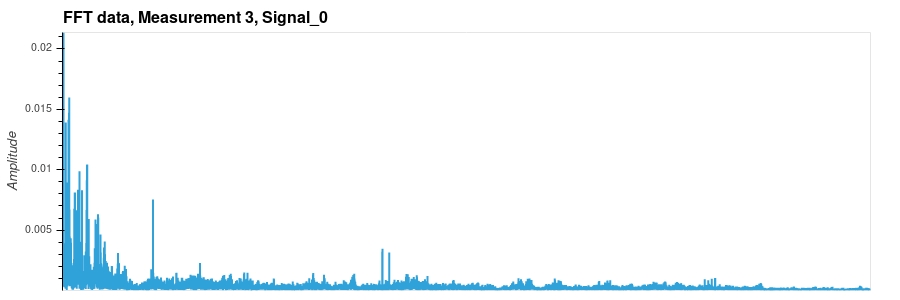
\includegraphics[width=\textwidth]{figures/Signal_0_fft_example.png}
\caption{Signal 0 fft example}
\end{subfigure}
%
\begin{subfigure}{0.9\textwidth}
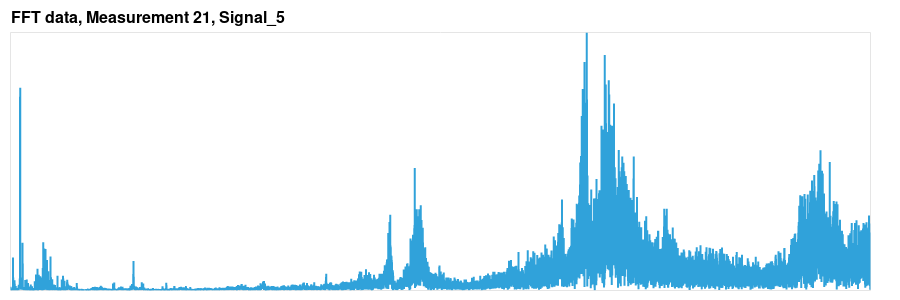
\includegraphics[width=\textwidth]{figures/Signal_5_fft_example.png}
\caption{Signal 5 fft example}
\end{subfigure}
\label{fft_example}
\end{figure}

Es wird sich zeigen, dass der Algorithmus für die dünnbesetzte Hauptkomponentenanalyse sehr rechenintensiv sein kann. Daher haben wir uns entschieden, nur einen Teil der ursprünglichen Zeitreihe zu verwenden. Abbildung REF rechtfertigt diesen Schritt. Hier sieht man, dass sich die Frequenzen über die Zeit kaum ändern, was daran liegt, dass der Maschine konstant Material zugeführt wird. Somit können wir die Dimension um einen Faktor $100$ reduzieren ohne wichtige Informationen zu verlieren. Des Weiteren wurden Teile der Frequenzen, welche außerhalb des Frequenzbereichs des jeweiligen Sensors liegen, abgeschnitten. Zu Schluss haben wir die Daten ähnlich wie bei der klassischen Hauptkomponentenanalyse zentriert, um die Varianzen der verschiedenen Frequenzen vergleichbarer zu machen.


%----------------------------------------------------------------------------------------
%	Anwedung auf Frequenzdaten
%----------------------------------------------------------------------------------------


\section{Anwendung auf Frequenzdaten}
\label{application_frequency_data}

Unsere Implementierung ermöglicht verschiedene Modellparameter zu wählen. Für eine Beschränkung der Laufzeit setzen wir eine maximale Anzahl an Iterationen von $500$ und eine Toleranz von $10^{-4}$. Falls nach $500$ Iterationen die vorgegebene Toleranz noch immer nicht erreicht ist, werden wir dies im Folgenden kenntlich machen. Ein weiterer Parameter den es zu wählen gilt, ist die Anzahl zu berechnender Hauptkomponenten. Wie bereits in \ref{sparse_pca_theorems} beschrieben, wird dazu meist die klassische Hauptkomponentenanalyse verwendet. Wir haben uns für Analysezwecke dazu entschieden einen Durchlauf mit $2$ und einen mit $10$ Hauptkomponenten zu starten. Interessanter ist die Wahl der Hyperparameter $\lambda$ und $\alpha$, welche wesentlichen Einfluss auf die Ergebnisse besitzen. Für die Wahl von $\lambda$ haben wir einerseits mehrere Werte ausprobiert, als auch eine Rastersuche bezüglich der in \ref{choice_of_tuning_parameters} beschriebenen BIC-Kriterien durchgeführt. Dafür verwenden wir auf einer log-Skala gleichverteilte Werte im Bereich zwischen $10^{-7}$ und $10^0$. Dagegen wählen wir für das Verhältnis zwischen Lasso und Ridge-Bestrafung die Werte $[0.1, 0.5, 0.7, 0.9, 0.95, 0.99, 1]$. Mithilfe der Kreuzvalidierung kann dann ein bester Wert für $\alpha$ bestimmt werden. Es hat sich in den Anwendungen gezeigt, dass eine geeignete Liste für $\alpha$ mehr Werte nahe bei $1$ hat, da sich dort die größten Änderungen ergeben. Damit stärken wir den Lasso-Strafterm im Vergleich zum Ridge-Strafterm. (Minimieren wir zeitgleich über $\lambda$ und $\alpha$

Exemplarisch werden wir uns nun mit einem der akustischen und einem der Beschleunigungssensoren weiter beschäftigen. An dieser Stelle möchten wir erwähnen, dass wir die Sensoren getrennt betrachten, d.h. die dünnbesetzte Hauptkomponentenanalyse auf die Sensoren einzeln anwenden. Dies ist aufgrund der Unterschiedlichkeit der Sensoren sinnvoll. Um einen Vergleich zu ermöglichen, haben wir zeitgleich die klassische Hauptkomponentenanalyse auf den Datensatz angewandt. Wir möchten nun ausgewählte Ergebnisse vorstellen. 


%----------------------------------------------------------------------------------------
%	Auswertung der Ergebnisse
%----------------------------------------------------------------------------------------


\section{Auswertung der Ergebnisse}
\label{evaluation}

Im Rahmen dieser Arbeit können wir nun einen begrenzten Teil der Ergebnisse vorstellen. Ziel wird es sein, alle wesentlichen Effekte zu erläutern und gegebenenfalls weiter ins Detail zu gehen. 


%----------------------------------------------------------------------------------------
%	Klassische Analyse der Hauptachsen
%----------------------------------------------------------------------------------------


\subsection{Klassische Analyse der Hauptachsen}

Zunächst wollen wir einen Blick auf die entstehenden Hauptachsen und Hauptkomponenten werfen. Dazu betrachten wir Abbildung REF, in welcher sowohl die klassischen als auch die dünnbesetzten Hauptachsen für zwei verschiedene Sensoren dargestellt sind. Anhand der Hauptachsen können wir erkennen, welche Frequenzen eine entscheidende Rolle bei der Erhaltung der maximalen Varianz spielen. Demnach sind die größten Unterschiede im Datensatz bei den Frequenzen mit der größten Werten in diesem Bild. In beiden Fällen besitzen die klassischen Hauptachsen $\approx20,000$ von Null verschiedene Einträge, auch wenn dies gerade für den akustischen Sensor schwer zu erkennen ist. Direkt darunter befinden sich die zugehörigen dünnbesetzten Hauptachsen, welche nur $1$ bzw. $\approx200$ von Null verschiedene Einträge besitzen. Wir haben daher eine wesentliche Reduktion in der Komplexität der Hauptachsen erreicht. Dies ist wichtig, wenn es darum geht die Ergebnisse zu interpretieren. Ein Blick auf Abbildung REF

\begin{figure}
\centering
%
\begin{subfigure}{0.9\textwidth}
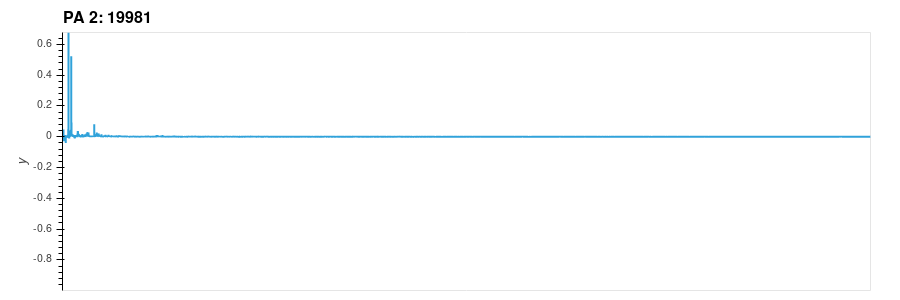
\includegraphics[width=\textwidth]{figures/Signal_0_principal_axis.png}
\caption{Signal 0 principal axis}
\end{subfigure}
%
\begin{subfigure}{0.9\textwidth}
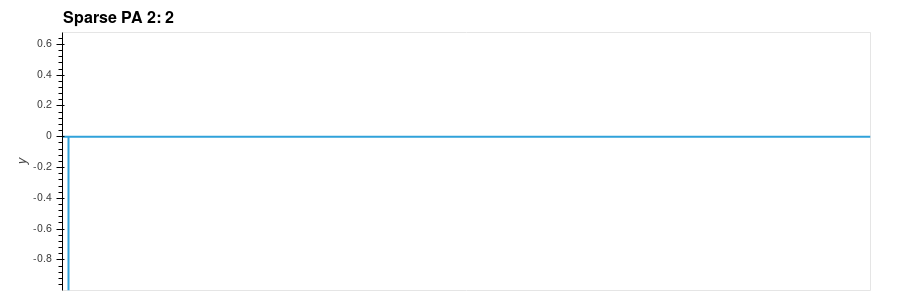
\includegraphics[width=\textwidth]{figures/Signal_0_sparse_principal_axis.png}
\caption{Signal 0 sparse principal axis}
\end{subfigure}
%
\begin{subfigure}{0.45\textwidth}
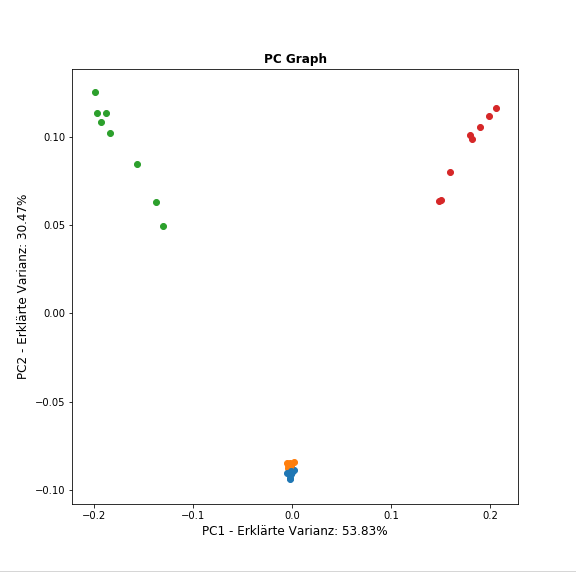
\includegraphics[width = \textwidth]{figures/Signal_0_pc_graph.png}
\caption{Signal 5 PC Graph}
\end{subfigure}
%
\begin{subfigure}{0.45\textwidth}
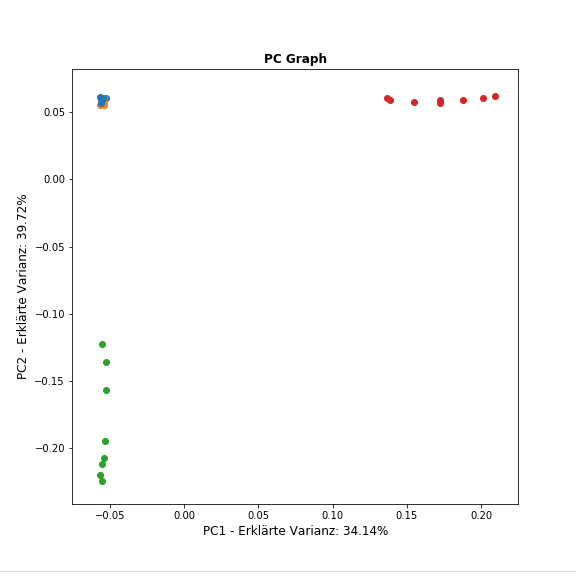
\includegraphics[width = \textwidth]{figures/Signal_0_sparse_pc_graph.png}
\caption{Signal 5 Sparse PC Graph}
\end{subfigure}
%
\begin{subfigure}{0.9\textwidth}
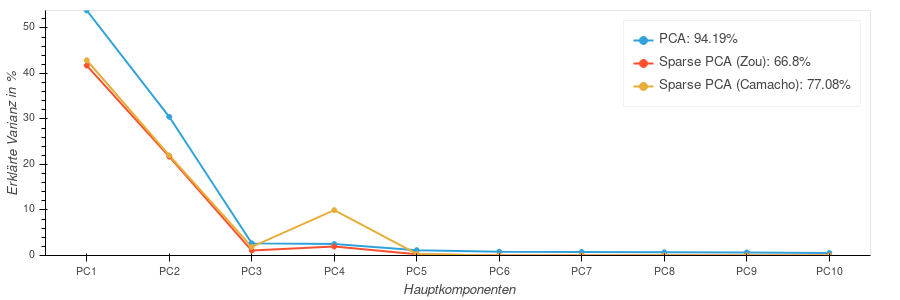
\includegraphics[width = \textwidth]{figures/Signal_0_scree_plot_10.png}
\caption{Signal 0 Scree Plot}
\end{subfigure}
\caption{Vergleich der klassischen mit der dünnbesetzten Hauptkomponentenanalyse für ein $\lambda=0.0001$ und $\alpha = 0.95$.}
\end{figure}

\begin{figure}
\centering
\begin{subfigure}{0.9\textwidth}
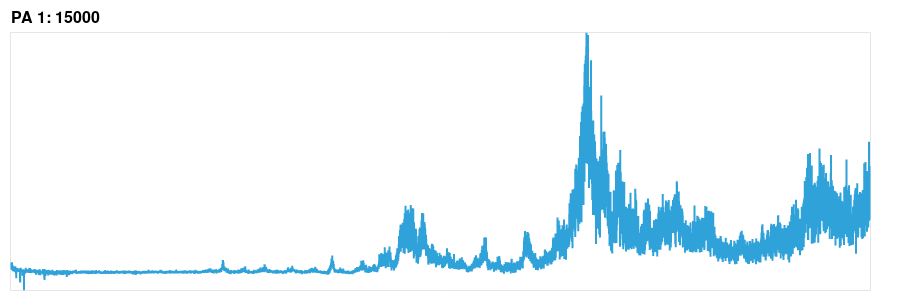
\includegraphics[width=\textwidth]{figures/Signal_5_principal_axis.png}
\caption{Signal 5 principal axis}
\end{subfigure}
%
\begin{subfigure}{0.9\textwidth}
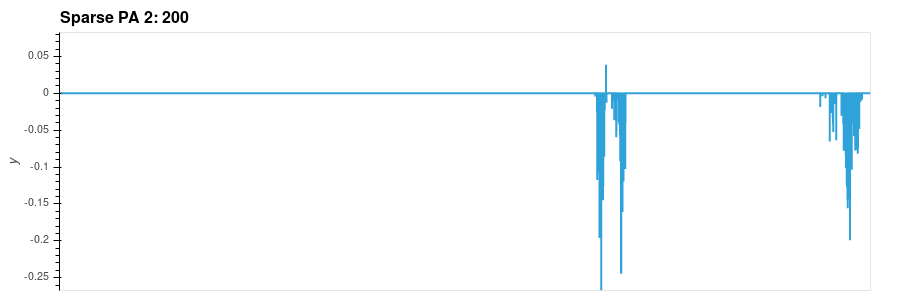
\includegraphics[width=\textwidth]{figures/Signal_5_sparse_principal_axis.png}
\caption{Signal 5 sparse principal axis}
\end{subfigure}
%
\begin{subfigure}{0.45\textwidth}
\centering
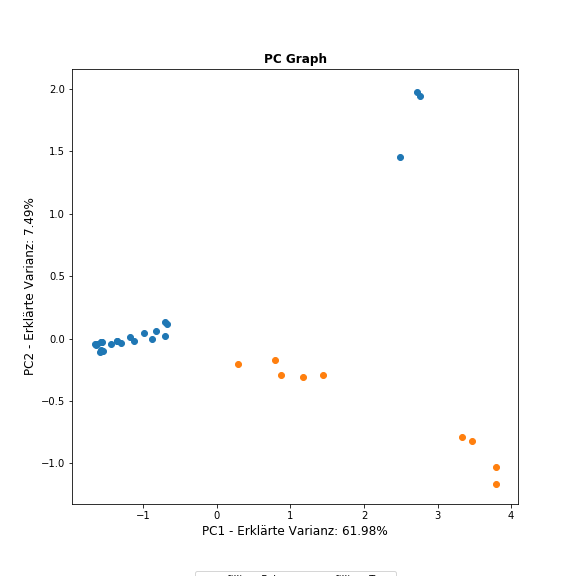
\includegraphics[width = \textwidth]{figures/Signal_5_pc_graph.png}
\caption{Signal 5 PC Graph}
\end{subfigure}
%
\begin{subfigure}{0.45\textwidth}
\centering
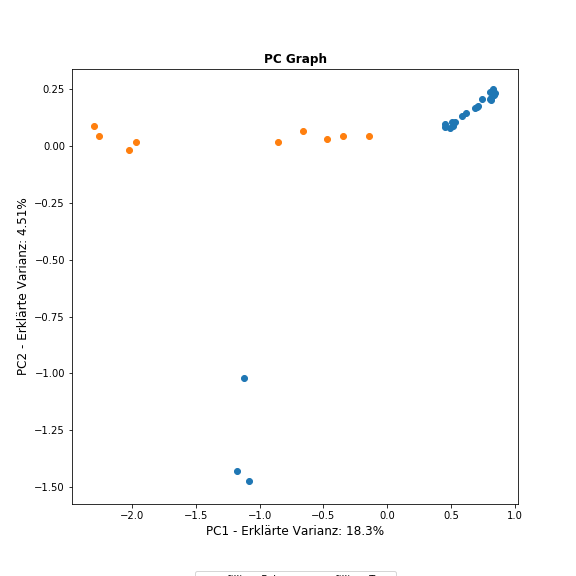
\includegraphics[width = \textwidth]{figures/Signal_5_sparse_pc_graph.png}
\caption{Signal 5 Sparse PC Graph}
\end{subfigure}
%
\begin{subfigure}{0.9\textwidth}
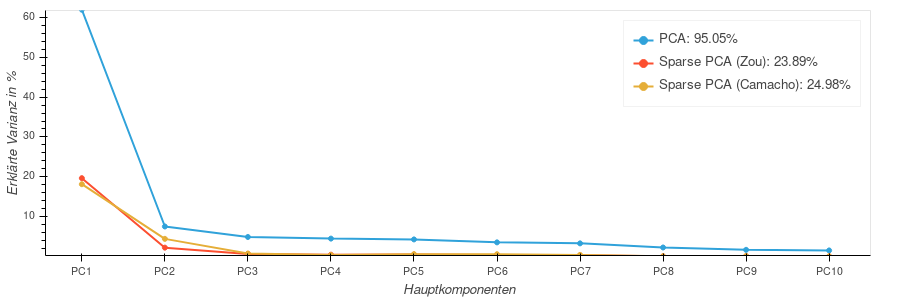
\includegraphics[width = \textwidth]{figures/Signal_5_scree_plot_10.png}
\caption{Signal 5 Scree Plot}
\end{subfigure}
\caption{Vergleich der klassischen mit der dünnbesetzten Hauptkomponentenanalyse für ein $\lambda=0.1$ und $\alpha = 0.1$.}
\end{figure}


%----------------------------------------------------------------------------------------
%	Wahl der Hyperparameter
%----------------------------------------------------------------------------------------


\subsection{Wahl der Hyperparameter}

Im vorangegangenem Abschnitt haben wir beispielhaft gezeigt, wie die Ergebnisse einer dünnbesetzten Hauptkomponentenanalyse zu interpretieren sind. Für die klassische Analyse haben wir bestimmte Werte von $\alpha$ und $\lambda$ vorgegeben, die möglichst gute Ergebnisse erzielen. Es stellt sich jedoch die Frage, wie sich die einzelnen Hauptachsen und Hauptkomponenten verändern, falls wir andere Werte für die Hyperparameter wählen. Zu diesem Zweck wenden wir uns Abbildung \ref{results_parameter_benchmark} zu. Hier haben wir versucht, die Effekte in Abhängigkeit von $\lambda$ zu beschreiben. Zuvor haben wir mithilfe der klassischen Hauptkomponentenanalyse und der Auswahlkriterien in Abschnitt \ref{selection_principal_components} festgestellt, dass für diesen Sensor mit $2$ Hauptachsen einen Großteil der Varianz erklären können. Daher haben wir diese Anzahl fixiert und nur $\lambda$ bzw. $\alpha$ variiert. 

Abbildung \ref{results_parameter_benchmark_degrees_of_freedom} zeigt wie sich $\operatorname{df}(\lambda)$, also die Anzahl von Null verschiedener Einträge in den Hauptachsen, bei Veränderung von $\lambda$ bzw. $\alpha$ verhält. Klar erkennbar ist der relativ gleichmäßige Abfall der Freiheitsgrade, d.h. für wachsendes $\lambda$ werden unsere Hauptachsen zunehmend dünnbesetzt. Dies entspricht unseren Erwartungen aus Kapitel \ref{sparse_pca}. Verschieben wir das Verhältnis der Bestrafung von der $\ell_1$ zur $\ell_2$-Norm, sprich kleineres $\alpha$ und mehr Gewicht auf der $\ell_2$-Norm, steigt die Anzahl der Freiheitsgrade. Dies bestätigt, dass die $\ell_1$-Norm im Gegensatz zur $\ell_2$-Norm eine Dünnbesetzung hervorruft. Ab einem gewissem Punkt $\lambda \approx 10^{-2}$ ist die Bestrafung zu stark, so dass die Hauptachsen dem Nullvektor entsprechen und keine Anpassung an den Datensatz mehr stattfindet.

Interessant ist nun, wie sich die erklärte Varianz des Datensatzes im Vergleich verhält, welche in Abbildung \ref{results_parameter_benchmark_explained_variance} zu sehen ist.  Auffällig ist, dass sich für $\lambda$ im Bereich von $[10^{-7}, 10^{-3}]$ kaum Änderungen in der Varianz ergeben. In diesem Bereich sind wir nur leicht unter dem Niveau der klassischen Variante. Im Umkehrschluss können wir aufgrund der kontinuierlichen Stagnation der Freiheitsgrade die Modellkomplexität verringern und zeitgleich den Rekonstruktionsfehler auf konstantem Niveau halten. Erst nahe $\lambda \approx 10^{-2}$ für $\alpha > 0.5$ bzw. bei $\lambda \approx 10^{-1}$ für $\alpha = 0.1$ zeichnet sich ein deutlicher Einbruch ab. Dieser ist dadurch zu erklären, dass die Hauptachsen dann dem Nullvektor entsprechen. Aus der Kombination der beiden Abbildungen können wir schließen, dass nur wenige Frequenzen wirklich wichtig zur Erklärung der Varianz des Datensatzes notwendig sind.

Um eine automatisierte Wahl von $\lambda$ und $\alpha$ zu ermöglichen, haben wir in Abschnitt \ref{choice_of_tuning_parameters} Vorgehensweisen mithilfe eines BIC-Kriteriums beschrieben. Eine Anwendung des Kriteriums nach \cite{croux, guo} befindet sich in Abbildung \ref{results_parameter_benchmark_bic}. Hier zeichnet sich ein Minimum im Bereich von $\lambda \in [10^{-4}, 10^{-3}]$ für $\alpha > 0.5$ bzw. nahe $\lambda \approx ^{-2}$ ab, welches wir nach obiger Analyse erwarten konnten. Es wird also ein Punkt gewählt, an welchem die erklärte Varianz gerade noch auf sehr hohem Niveau, aber die Modellkomplexität gering ist. Letztere Abbildung ist also eine Kombination der Erkenntnisse.

\begin{figure}
\centering
\begin{subfigure}{0.9\textwidth}
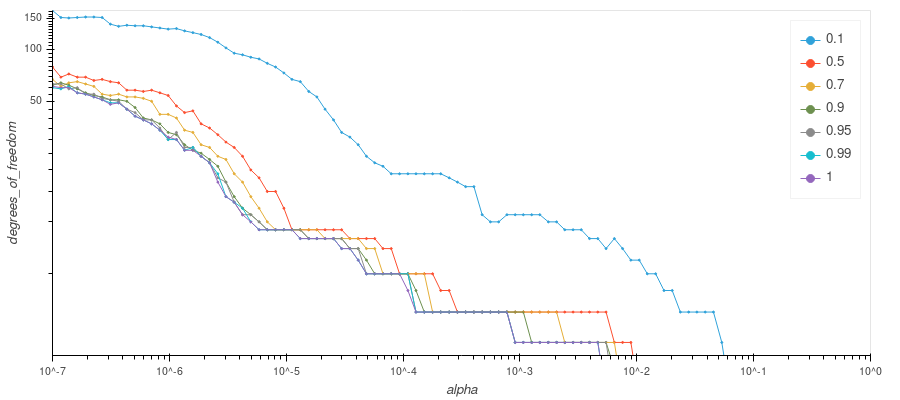
\includegraphics[width=\textwidth]{figures/Signal_0_degrees_of_freedom.png}
\caption{Anzahl Freiheitsgrade in Abhängigkeit von $\lambda$.}
\label{results_parameter_benchmark_degrees_of_freedom}
\end{subfigure}
%
\begin{subfigure}{0.9\textwidth}
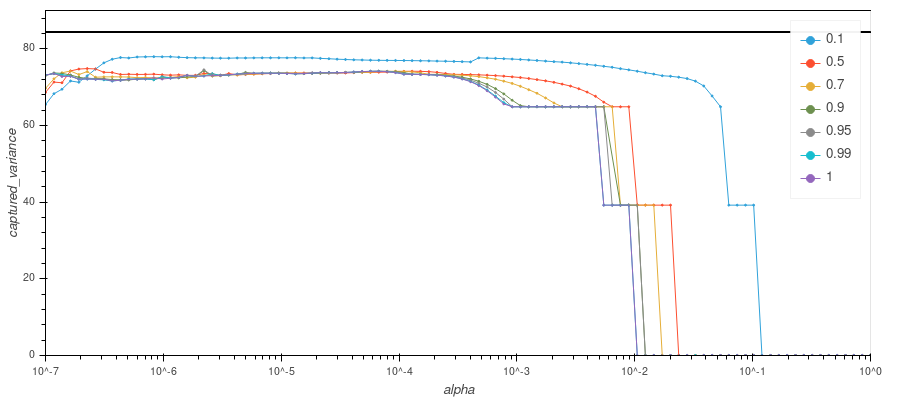
\includegraphics[width=\textwidth]{figures/Signal_0_explained_variances.png}
\caption{Erklärte Varianz des Datensatzes in Abhängigkeit von $\lambda$.}
\label{results_parameter_benchmark_explained_variance}
\end{subfigure}
%
\begin{subfigure}{0.9\textwidth}
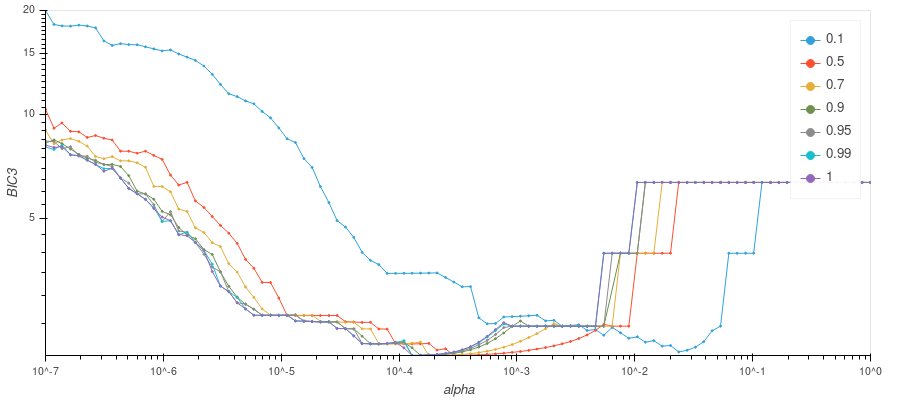
\includegraphics[width=\textwidth]{figures/Signal_0_bic.png}
\caption{Wahl der Hyperparameter mithilfe eines minimalen BIC-Kriteriums.}
\label{results_parameter_benchmark_bic}
\end{subfigure}
\caption{Die Abbildung zeigt wie sich eine Wahl der Hyperparameter $\alpha$ und $\lambda$ mithilfe eines BIC-Kriterium gestalten kann. Um Erkenntnisse über die Entstehung der BIC-Abbildung zu gewinnen, werden zusätzlich die beiden Komponenten Anzahl Freiheitsgrade und erklärte Varianz gezeigt. Zu beachten ist die logarithmische Skala für $\lambda$.}
\label{results_parameter_benchmark}
\end{figure}


%----------------------------------------------------------------------------------------
%	Verhalten des Algorithmus
%----------------------------------------------------------------------------------------


\subsection{Verhalten des Algorithmus}

Im Zuge dieser Arbeit möchten wir nicht nur die Ergebnisse einiger Experimente, sondern auch das Verhalten des Algorithmus an sich beschreiben. Dafür werden wir uns verschiedene Größen wie Laufzeit, Anzahl Iterationen und Toleranz ansehen. 

Gerechnet wurde auf Intel Xeon Gold 6130F@2.10GHz.

Laufzeit pro Iteration erhöht sich mit $\alpha$.
\begin{figure}
\centering
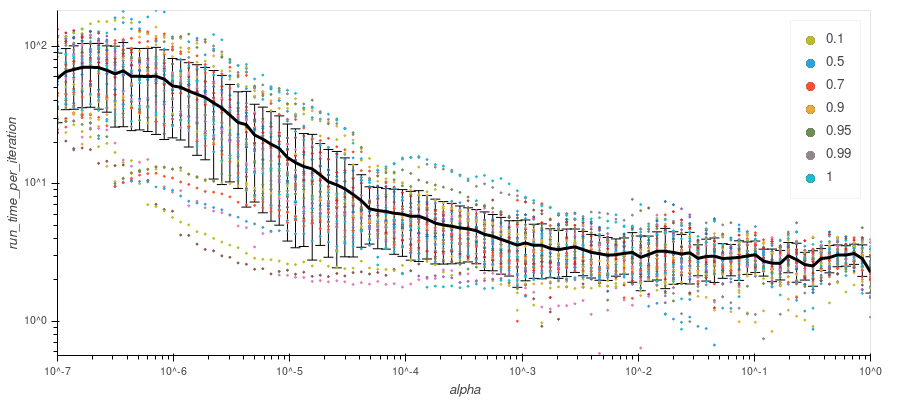
\includegraphics[width = 0.9\textwidth]{figures/run_time_per_iteration.png}
\caption{In dieser Abbildung ist die Laufzeit pro Iteration bei Veränderung des Hyperparameters $\lambda$ auf einer logarithmischen Skala zu sehen. Da auch $\alpha$ in unseren Experimenten variiert worden ist und mehrere Sensoren betrachtet werden, sehen wir mehrere Punkte je $\lambda$. Im Mittel klar zu erkennen ist ein Anstieg der Laufzeit bei Verringerung der Stärke der Bestrafung $\lambda$.}
\label{run_time_per_iteration}
\end{figure}

Anzahl an Iterationen mit $\alpha$?


%----------------------------------------------------------------------------------------
%	Experimentelle Überprüfung der berechneten Varinanz
%----------------------------------------------------------------------------------------


\subsection{Experimentelle Überprüfung der berechneten Varianzen}

In Abschnitt \ref{adjustment_of_variances} haben wir unterschiedliche Wege zur Berechnung der Hauptkomponenten und deren erklärte Varianz gezeigt. Um die Arbeit von Camacho et al. \cite{camacho} experimentell zu überprüfen, werden wir vier Kriterien definieren, welche auf den unterschiedlichen Vorgehensweisen basieren. Für jede dieser wird die Varianz der Residuen addiert und mit der Gesamtvarianz des Datensatzes normalisiert.
\begin{itemize}
\item TotQR: $\quad \frac{\sum_{j=1}^k R_{jj}^2 + \spur{\mat E^T\mat E}}{\spur{\mat X^T\mat X}} \quad$ (Vorgehensweies Zou et al.)
\item TotZB: $\quad \frac{\spur{\mat B \mat Z^T \mat Z \mat B^T} + \spur{\mat E^T\mat E}}{\spur{\mat X^T\mat X}} \quad$ (Vorgehensweise Camacho et al.)
\end{itemize}
Bezüglich der Notation haben wir uns an Abschnitt \ref{adjustment_of_variances} gehalten. Zwei weitere Kriterien TotQR* und TotZB* ergeben sich durch die Korrektur der Hauptkomponenten mit der Moore-Penrose-Inverse $\mat Z^* = \mat X \mat B^T (\mat B^T\mat B)^+$. Falls alle Vorgehensweisen korrekt sind, können wir erwarten, dass jedes Kriterium den Wert $1$ hat. In Abbildung \ref{total_variance_validation} haben wir die Kriterien für unsere Experimente berechnet. Klar zu sehen ist, dass ohne eine Korrektur mit der Moore-Penrose-Inversen beide Varianten für die Varianzberechnung im Allgemeinem falsch sind. Auch wenn wir die Hauptkomponenten korrigieren, liefert die QR-Zerlegung keine richtigen Ergebnisse. Nur TotZB* hat in allen Fällen den Wert $1$ und ist damit der korrekte Weg, Hauptkomponenten und Varianzen zu berechnen. Somit können wir die Erkenntnisse aus \cite{camacho} experimentell bestätigen.

\begin{figure}
\centering
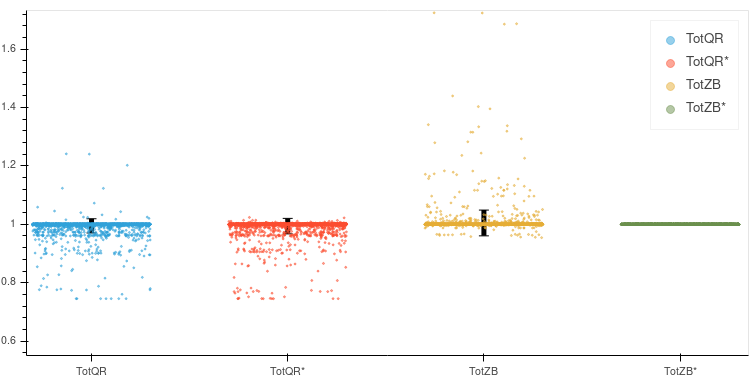
\includegraphics[width = 0.9\textwidth]{figures/total_variance_validation.png}
\caption{Zu sehen sind die Ergebnisse der unterschiedlichen Vorgehensweise bei der Berechnung der Hauptkomponenten und erklärter Varianzen. Nur die von Camacho et al. vorgeschlagene Variante TotZB* errechnet diese korrekt. Jeder Punkt entspricht eines unserer Experimente wie in Abschnitt \ref{application_frequency_data} beschrieben.}
\label{total_variance_validation}
\end{figure}